\chapter{Machine learning: an overview}
\label{chp:ml}
This chapter is dedicated to the theoretical exploration of some of the most important concepts in
machine learning alongside the various models that have been used in the project. We will begin with
a concise explanation of the more basic concepts linked to machine learning, then we will move to a
theoretical overview of the supervised models used for the project, followed by a brief introduction to
unsupervised machine learning models.

\section{Supervised machine learning}
\label{sec:sml}
Due to the popularization of artificial intelligence in recent times, it's very important to establish the field to avoid the risk of
incurring in misunderstandings. \emph{Machine learning} is a subset of artificial
intelligence, and is a technique that allows us to solve a problem without the need to actually invent an
algorithm to solve it (as long as there is enough data). There are many different problems that
either lack an algorithmic solution or have an inefficient one; in such cases, machine learning is
an alternative worth exploring. The tradeoff of using machine learning instead of 'classic'
problem-solving techniques is that the solution is built using heuristic methods,
therefore is not \emph{correct} for the problem \cite{Rebala2019}.

\medskip

A supervised machine learning model is a model $\model$ capable of learning a mapping between the
input space $\ins$ and the output space $\outs$ and then apply this mapping to unseen
data to predict the output \cite{Cunningham2008}.

\smallskip

Given a problem $\problem$, a specific instance of $\problem$, $\problem_i$, is characterized by a pair
$(\vec{x}_i, y_i)$ where $\vec{x}_i \in \ins$ are vectors taken from an input space $\ins$, usually
highly dimensional, and $y_i \in \outs$ are the expected solutions, which can be scalar or
vector\footnote{Outcomes will be considered scalars for the rest of this thesis unless explicitly
	stated}. The single components of every input vector, $\vec{x}_i$, are called
\emph{features}, and are values (numerical or other) representing a particular aspect of the domain.

A \emph{dataset} is a set containing $m$ problem instances $\dset$, and
a supervised machine learning model $\model$, trained on $D$, can be used to predict the outcome,
$\hat{y}$, of any instance of the problem $\problem_i$. Note that a machine learning model is the result of a
statistical process, therefore is susceptible to change unless the randomicity is kept under control.
On a practical level we can make sure that, for reproducibility purposes, the random number
generators associated to the various libraries are set to a definite value.

\medskip

To clarify the concepts just introduced, let us consider the following mock-problem: 'Is it going to rain
tomorrow?'. The dataset $D$ contains $365$ instances of the problem, one per day, for a year. The
input vector for every problem is a set of atmospheric measurements (e.g., temperature, atmospheric
pressure, exposure, humidity, \ldots), each measurement a different feature of the dataset. The
output of every instance $\problem_i$ is a flag answering the question 'did it rain on day $i$?'
with a $1$, for True, and a $0$, for False.

Due to the high grade of complexity of the problem solved in this thesis, future concepts will be clarified
using this exact mock-problem or its variations.

\medskip

In general, a machine learning problem can be defined as the process of finding the mapping that
relates the input space $\ins$ to the output space $\outs$ by abstracting patterns from
a training set. Conventionally, the output space can be interpreted differently based on
the problem:
\begin{itemize}
	\item $\outs = \{-1, 1\}$, for \emph{binary classification} problems, which are usually
	      associated with pattern recognition tasks, a very easy example of binary classification is our mock-problem.
	\item $\outs = \{a_1,\ldots, a_m\}$, for \emph{multi-class classification} problems, in
	      which an element can be part of one of the classes in a certain set, a classic
	      example is the character recognition problem, in which a certain character given in input can belong to one of 10 different classes (the numbers from 0 to 9) \cite{pal2010handwritten}.
	\item $\outs = \mathbb{R}$, for \emph{regression problems}, which are usually associated
	      with function approximation tasks, an example of regression problem
	      is: 'Based on the current amount of wins for Oklahoma City Thunder\footnote{An
		      amazing \textsc{nba} team}, predict the team's win rate at the end of the season'.
\end{itemize}

Most machine learning models have to go through the same steps, described here below
\begin{itemize}
	\item \emph{Model selection}: if we consider an instance of a decision tree (introduced in
	      \Cref{sec:dt}), the model can be described through a set of characteristics (e.g.,
	      number of nodes, depth, splitting method, \ldots), all of these are known as
	      \emph{hyperparameters}. An important step of solving a machine learning problem is
	      doing an exploration, even if not thorough, due to the exponential complexity of the
	      task, of the hyperparameter space, to find the best possible combination for the
	      problem.
	\item \emph{Model training}: during the training procedure, the instance of the model abstracts
	      patterns from a sample of the dataset, which we will call \emph{training set} $T$.
	\item \emph{Model testing}: during the testing procedure the model performance is tested on a
	      part of the dataset, which we will call \emph{test set} $G$ (standing for
	      \emph{generalization}). This set is used to understand whether the performance found for model
	      $\model$ is a statistical anomaly (therefore depending on the points
	      chosen to build $T$) or extends also to unseen data.
\end{itemize}

There are many different approaches to splitting a dataset $D$ into a series of separate parts
for the various tasks involved in the machine learning problem resolution (e.g., model training,
model testing, model selection, \ldots). In the following I will describe two non-trivial aspects of
the basic procedure to split a dataset $D$ into a training dataset $T$ and a testing dataset $G$ and a
more complex splitting procedure will be introduced at a later time.

\medskip

As a first non-trivial aspect of the splitting procedure is that, depending on the problem, making
sure that the distribution of training dataset $T$ and testing dataset $G$ is the same as the
original dataset distribution is important. To understand why, let's think about a dataset
$\dset$ in which every $\mathbf{x}_i \in \ins$ is a vector of features describing a patient's
conditions (e.g., age, sex, body temperature, blood saturation, \ldots) and every $y_i \in \outs$ is
a string indicating which illness was diagnosed (e.g., flu, pneumonia, \textsc{covid}, ...). Supposing we want to find a
model $\model$ capable of doing a diagnosis effectively: we need to make sure that the least
represented illnesses (which are usually the more dangerous ones) are well represented in both $T$
and $G$. If this splitting process was not done correctly we might end up with a model $\model$ that
can reliably recognize a common flu but can't correctly identify serious illnesses like pneumonia.

\medskip

The second non-trivial aspect of the splitting procedure is that it's always necessary to make sure
that the operation is carried out independently for each dataset, this means that data that is in the
training set cannot be in the testing set, and vice versa. If this were not to be true then we would
have a data leak from one set to the other.

\smallskip

Whenever a data leak is identified from the training set $T$ to the testing set $G$, some points
that were used to train $\model$ are used once more to test its performance, which leads to a higher
performance metric, relaying higher and unjustifed confidence in the model performance.

\medskip

To close this section about supervised learning, we will be introduced to two issues specific to
supervised learning models. Whenever we work in the field of supervised learning it's important to be aware of two classic issues: \emph{overfitting} and \emph{underfitting}.

\smallskip

Given the generic machine learning problem $\problem$ and a dataset $\dset$, the model $\model$ that
solves $\problem$, is said to be overfitting when the training performance is acceptable, but the
testing performance is unacceptably bad; this means that the mapping found by $\model$ to link $\ins$
and $\outs$ is too closely related to the specific data chosen to do the training, therefore
unable to generalize effectively. In other
words, $\model$ is overfitting whenever, instead of abstracting some general patterns in the
data, it actually learns some peculiarities of the specific training dataset $T$ \cite{ZhouZhi-Hua2021ML}
which are not found later in the testing dataset $G$.

\smallskip

An 'orthogonal' problem to overfitting is the issue of \emph{underfitting}, which is usually caused
by a model not being powerful enough to abstract information from a certain dataset. Whenever a
machine learning model is underfitted for a problem $\problem$, the performance metrics obtained
during training and testing are unacceptably bad, independently of the train and test set
utilized.

\medskip

The problem that this thesis aims to solve takes full advantage of supervised models, since the data at our
disposal has already been analyzed and labelled in previous works \cite{mariotto2022}\cite{mariotto2022-generic}.

\medskip

In the following we will be discussing, on a theoretical level, the various supervised models deployed
to solve the problem.

\section{Decision Trees}
\label{sec:dt}
This section is a theoretical introduction to decision trees, the implementation we used for the
model is the \emph{DecisionTreeClassifier} class contained in scikit-learn.

\medskip

A decision tree is a machine learning model based on a tree structure, an example of such a
structure can be seen in \Cref{fig:simple-dt}. Each internal node contains a condition that needs to
be evaluated on one or more features (e.g.,  the root of \Cref{fig:simple-dt} requires us to check
whether the humidity feature of the input is $\geq 80\%$), if the result of the evaluation is true
the computation proceeds with the left child, otherwise the right path will be taken. Once a leaf is
reached, the class associated to the point is identified. If we consider again \Cref{fig:simple-dt}
we could say that if the humidity of the input is $\geq 80\%$ and the temperature is $\geq 10C$ then
the inputs will be classified as 'rain'.

Any path leading from root to leaf is known as a \emph{decision path}. It's evident that such structures have a very high degree of explainability and that is why usually they are the first model chosen to solve a machine learning problem.

\medskip

Two are the theoretical concepts I wish to cover in this section: indices and node split
computation, avoiding overfitting through pre- and post- pruning.
\begin{figure}
	\centering
	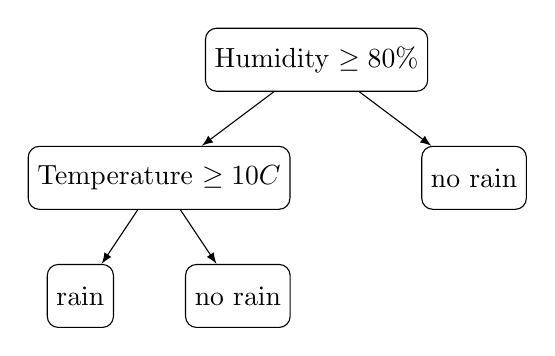
\begin{tikzpicture}[
			% Define styles for nodes
			level 1/.style={sibling distance=40mm},
			level 2/.style={sibling distance=20mm},
			level 3/.style={sibling distance=10mm},
			every node/.style={draw, rectangle, rounded corners, align=center, minimum size=8mm},
			edge from parent/.style={draw, -latex}
		]

		% Root node
		\node {Humidity $\geq 80\%$}
		% First level
		child {node {Temperature $\geq 10C$}
				% Second level
				child {node {rain}}
				child {node {no rain}}
			}
		child {node {no rain}};
	\end{tikzpicture}
	\caption{A very simple example of decision tree built on the mock problem}
	\label{fig:simple-dt}
\end{figure}
\subsection{Indices and node split computation}
In \Cref{fig:simple-dt} a simple structure for a decision tree was shown, an excellent question in
its regard could be: 'Why this structure and not another one?'. Other than it being a simple example
nothing is really preventing us from describing the 'rain' event based on different threshold values
or different feature sets altogether.
\begin{figure}
	\centering
	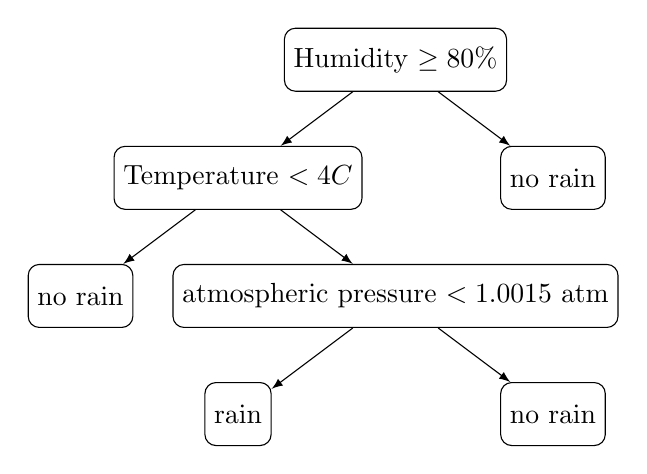
\begin{tikzpicture}[
			% Define styles for nodes
			level 1/.style={sibling distance=40mm},
			level 2/.style={sibling distance=40mm},
			level 3/.style={sibling distance=40mm},
			every node/.style={draw, rectangle, rounded corners, align=center, minimum size=8mm},
			edge from parent/.style={draw, -latex}
		]

		% Root node
		\node {Humidity $\geq 80\%$}
		% First level
		child {node {Temperature $< 4C$}
				% Second level
				child {node {no rain}}
				child {node {atmospheric pressure $< 1.0015$ atm}
						child{node {rain}}
						child{node {no rain}}
					}
			}
		child {node {no rain}};
	\end{tikzpicture}
	\caption{Another decision tree built on the mock-problem and alternative to
		\Cref{fig:simple-dt}}
	\label{fig:simple-dt-alt}
\end{figure}
The mock tree shown in \Cref{fig:simple-dt-alt} is a different tree compared to the one shown in
\Cref{fig:simple-dt} and yet they solve the same problem by characterizing it differently.
\Cref{algo:decision-tree} shows how the decision tree is built, line $9$ states that the best
splitting feature needs to be selected with every iteration, this choice is taken based on a
\emph{purity} index applied to nodes.

\begin{algorithm}
	\caption{The decision tree base algorithm taken from
		\cite{ZhouZhi-Hua2021ML}}\label{algo:decision-tree}
	\begin{algorithmic}[1]
		\Require Training set $\dset$ and Feature set $A = \{a_1, \ldots,
			a_d\}$.
		\Ensure A decision tree
		\Function{TreeGenerate}{$D$, $A$}
		\State Generate node $i$;
		\If{All samples in $D$ belong to the same class $C$}
		\State Mark node $i$ as a class $C$ leaf node; \textbf{return node $i$}
		\EndIf
		\If{$A = \emptyset$ \textsc{or} all samples in $D$ take the same
			value on $A$}
		\State Mark node $i$ as a leaf node, its class label is
		the majority in $D$;
		\State \textbf{return node $i$}
		\EndIf
		\State Select the optimal splitting feature $a_*$ from $A$;
		\For{each value $a_*^v$ on $a_*$}
		\State Generate a branch for node $i$;
		\State Let $D_v$ be the subset of samples taking value $a_*^v$ on $a_*$;
		\If{$D_v$ is empty}
		\State Mark this child node as a leaf node;
		\State label t with the majority class of $D$;
		\textbf{return node $i$}
		\Else
		\State use \textproc{TreeGenerate}$(D_v, A \setminus \{a_*\})$ as the child node.
		\EndIf
		\EndFor
		\EndFunction
	\end{algorithmic}
\end{algorithm}

\medskip

The purity of a node defines how heterogeneous are the samples associated to it. Intuitively, in the
context of our mock-problem: if the distribution of samples arriving to a node $i$ is $15$ labelled
$1$, and $1$ labelled $0$, then the purity of the node is going to be very high.

A split is going to be performed on feature $a$ only if the resulting purity increase is the best
possible. There are many different indices used to compute purity, in the following I will be
considering only the ones important for the model selection process that will be introduced in
a future chapter: \emph{Entropy} and \emph{Gini index}.

\subsubsection{Entropy}
There are many different ways of defining information entropy, a more general definition, compared
to the one found in \cite{ZhouZhi-Hua2021ML}, is found in \cite{gray2011entropy}. Let's consider a
random variable $f$ built on the alphabet $B = \{b_1, \ldots, b_{|B|}\}$ we can define the
partition $\mathcal{Q} = \{Q_i: i = 1, \ldots, |B|\}$ where $Q_i = \{\omega: f(\omega) = b_i\} = f^{-1}(b_i)$ therefore $\mathcal{Q}$ is a partition of the bigger
probability space $\Omega$, every partition is chosen based on the outcome of the
measurement of the random variable $f$. In the case of a discrete random variable we can define the
information entropy as shown in \Cref{eq:information-entropy}
\begin{equation}
	\label{eq:information-entropy}
	H_p(\mathcal{Q}) = - \sum_{i = 1}^{|B|}{P(Q_i)\log{P(Q_i)}}
\end{equation}
this definition of entropy can be easily extended to the dataset case since:
\begin{itemize}
	\item The partition set $\mathcal{Q}$ can be mapped to the dataset $D$,
	\item Every partition $Q_i$ can be mapped to the single class of the machine learning
	      problem that is being considered,
	\item The alphabet $B$ can be mapped to the set of possible outcomes of the machine learning
	      problem.
\end{itemize}
Therefore, we can rewrite \Cref{eq:information-entropy} as:
\begin{equation}
	H_p(D) = - \sum_{k = 1}^{|\outs|}p_k \log{p_k}
\end{equation}
$p_k$ denotes the proportion of the $k$-th class inside dataset $D$.

If we consider the binary classification problem ('true' or 'false' response), whenever a splitting procedure
is done on a node in the tree, the split is computed on every feature based on the possible
values of the feature itself (only for discrete features), if we consider our mock-problem, a split could be computed on a
feature called  'status of the sky' which can have one of two values $\{\text{overcast},
	\text{clear}\}$ the new node could be built in two different ways and
the class distribution for each is different, having different levels of purity based
on how well the data is partitioned between the classes 'rain' and 'no rain'.

\smallskip

To choose which of the two nodes to take in our mock-problem using the entropy measure we need to
introduce the concept of \emph{information gain}, which is expressed as follows:
\begin{equation}
	\label{eq:information-gain}
	\textsc{Gain}(D, a) = H_p(D) - \sum_{v = 1}^V\frac{|D^v|}{|D|}H_p(D^v)
\end{equation}
The concept expressed by information gain in \Cref{eq:information-gain} is that the amount of
information gained by doing a split of dataset $D$ on feature $a$ is given by the entropy of dataset
$D$ at the moment of the split from which we remove the entropy of the dataset resulting from the
split of feature $a$ at every value $v$ scaled by the ratio between the cardinality of the new dataset to
the cardinality of the original dataset.

\smallskip

The feature used to perform the actual splitting is going to be the one with the highest possible
information gain. It's very important to notice that information gain is an index biased towards
features that have many different values (and therefore $|D^v|$ is small). In the case of our mock
problem, if we consider 'status of the sky' and we compare it to another feature containing many
different splitting values for example 'cloud color' which might assume the following values
$\{\text{white}, \text{light grey}, \text{grey}, \text{black}, \text{pink}, \text{orange},
	\text{red}\}$ it's clear that the $|D^v|/|D|$ is going to be lower for each of them, therefore
leading to a lower entropy decrease and a higher information gain.

\medskip

The alternative to using information gain is to use the \emph{gain ratio}
\begin{equation}
	\label{eq:gain-ratio}
	\textsc{GainRatio}(D, a) = \frac{\textsc{Gain}(D, a)}{\textsc{iv}(a)}
\end{equation}
the \textsc{iv} function in \Cref{eq:gain-ratio} is the \emph{intrinsic value} of feature $a$ and
can be computed as shown in \Cref{eq:intrinsic-value}.
\begin{equation}
	\label{eq:intrinsic-value}
	\textsc{iv}(a) = - \sum_{v = 1}^V\frac{|D^v|}{|D|} \log{\frac{|D^v|}{|D|}}
\end{equation}
Due to how intrinsic value is defined the gain ratio corrects the bias of the information gain towards features
with a higher number of values but is biased towards features with a lower amount of variables
\cite{ZhouZhi-Hua2021ML}.

In the actual implementation of the decision tree provided by scikit-learn an optimized version of
the \textsc{cart} algorithm is used, which  is similar to the \textsc{c4.5} algorithm proposed by Quinlan in
\cite{quinlan2014c4}.

\subsubsection{Gini index}
The original \textsc{cart} algorithm conceptualized by Breiman et al. in 1984
\cite{breiman1984classification} used Gini index to compute the best splitting feature for every
node. The Gini value of a dataset can be computed as shown in \Cref{eq:gini-value}
\begin{equation}
	\label{eq:gini-value}
	\textsc{Gini}(D) = \sum_{k = 1}^{|\outs|}\sum_{k' \neq k} p_kp_{k'} = 1 - \sum_{k =
		1}^{|\outs|}p_k^2
\end{equation}
As explained in \cite{ZhouZhi-Hua2021ML}, \Cref{eq:gini-value} can be interpreted as the
likelihood of taking samples from two different classes by drawing them randomly from the
dataset, the lower the $\textsc{Gini}(D)$, the higher the purity of a node. Gini index can be
computed as the weighted sum of all the Gini values for the dataset after the split, as shown in
\Cref{eq:gini-index}.
\begin{equation}
	\label{eq:gini-index}
	\textsc{GiniIdx}(D) = \sum_{v = 1}^V\frac{|D^v|}{|D|} \textsc{Gini}(D^v)
\end{equation}

The best splitting feature is going to be the one with the smallest Gini index overall.

\subsection{Avoiding overfitting through pre- and post- pruning}
As was argued in the previous section decision trees have an extremely simple structure and the
results are easy to interpret, since all we have to do is read the decision path for the samples of
interest.

Overfitting is probably the biggest drawback of decision trees, as shown in
\cite{overfitting-dt-erblin}, since the model tries to partition the space based on the purity of
the nodes, it's important to make sure that the splitting rules utilized are not overly specific.
Two techniques are commonly explored in the literature to prevent overfitting: \emph{pre-pruning}
and \emph{post-pruning}.

\medskip

Pre-pruning forces an early stop of the algorithm whenever a series of conditions allow it. The
definition of pre-pruning in the literature is a bit confusing, \comment{in some cases it's regarded as an
early stopping technique that only considers the impurity decrease}{Check
that the book actually says this (can't trust myself with this)} \cite{ZhouZhi-Hua2021ML}, in some
other cases, pre-pruning is defined as a group of techniques meant to keep the size of the decision
tree in check \cite{bramer2007principles}\cite{fisher1996learning}. The better definition is the
second one, since many splits reduce the impurity but introduce unwanted complexity in the model (e.g., because they are splitting a very small amount of samples, because the tree is already very deep, etc...).

\smallskip

The specific pre-pruning conditions that can be checked using the DecisionTreeClassifier class provided by
scikit-learn are the following:
\begin{itemize}
	\item The tree \emph{depth}, avoiding a complex tree structure by cutting the depth is
	      probably one of the easiest forms of pre-pruning.
	\item The \emph{impurity decrease} stops nodes from splitting when the decrease in impurity
	      of the children is not higher than a certain threshold, if the threshold is too high
	      then the tree will probably underperform, if it's too low then the tree is likely going to
	      overfit.
	\item The \emph{number of elements to split}, is basically a check that can be done on the
	      number of samples inside a node. An excellent way of avoiding overfitting is to not split a node containing few samples.
\end{itemize}

\medskip

Post-pruning is the alternative to pre-pruning, the essential difference between the two is that
post-pruning is done after the tree has been fully constructed. In the a posteriori phase,
a series of branches will be chosen to be pruned based on the impurity decrease that they provide.
There are different post-pruning techniques that can be implemented, scikit-learn is working with
Cost Complexity Pruning (\textsc{ccp}), introduced in \cite{breiman1984classification}.

\section{Ensemble learning}
\label{sec:el}
In the previous chapter I introduced decision trees, and we have talked at length about their
strength and weaknesses, providing some instruments to counter their shortcomings. Sometimes,
despite our efforts, the decision tree model is simply not enough for the task at hand, if we don't
want to give up the high explainability of tree models, in favor of higher performance, we can think
of creating an ensemble.

An ensemble is constructed by grouping weaker learners, which produces two main effects (to
clarify the concepts we will consider a basketball roster):
\begin{itemize}
	\item Different learners are able to grasp different sides of the problem, which would be
		either impossible or complicated for single models, if we consider our example, each
		player covers different positions which do not fit the other players (this doesn't
		mean that key players or superstars cannot play in other positions due to their
		performance).
	\item Using a group of models alleviates the shortcomings of the weaker links in the chain,
		if we consider our example, the weaker players, and lesser role players, can stay on the bench while the
		main rotation is playing, but can still contribute with some quality minutes when
		the main rotation is facing a difficulty.
\end{itemize}

Following the analysis done in \cite{ZhouZhi-Hua2021ML}, I will now prove that the error rate of a
binary classifier based on an ensemble of models falls to zero exponentially with the number of individuals
used.

Let's suppose that the error rate of each model in the ensemble is $\epsilon$, the ground truth
function is $f$ and the single learner is $h_i$, then we can express the probability of the learner
making a wrong prediction on $\vec{x} \in \ins$ as shown in \Cref{eq:error-rate}.
\begin{equation}
	\label{eq:error-rate}
	P(l_i(\vec{x}) \neq f(\vec{x})) = \epsilon
\end{equation}
Assuming that the prediction is $y \in \{-1, +1\}$, let's consider an ensemble in containing $T$
base learners, independent of each other, the ensemble will aggregate the predictions by using a
simple majority algorithm (\Cref{eq:ensemble-aggregation}).
\begin{equation}
	\label{eq:ensemble-aggregation}
	F(\vec{x}) = sign\left(\sum_{i = 1}^{T}l_i(\vec{x})\right)
\end{equation}
Since the probability of a base learner of being correct is $1 - \epsilon$, then the ensemble
correctly classifies a sample only if more than half of the learners correctly identify the sample.
This is expressed by \Cref{eq:succ-probability}.
\begin{equation}
	\label{eq:succ-probability}
	\begin{aligned}
		Pr(\text{success}) & = Pr\left(\text{at least } \left\lceil{\frac{T}{2}}\right\rceil \text{ correctly identify
		the sample}\right)
		\\
			   & = \sum_{k = \lceil{T / 2}\rceil}^T \binom{T}{k} (1 - \epsilon)^k
			   \epsilon^{T - k}
	\end{aligned}
\end{equation}
Since we are interested in finding a bound for ensemble error rate we are interested in the
complement of $Pr(\text{success})$, which is $Pr(\text{insuccess}) = Pr(F(\vec{x}) \neq
f(\vec{x}))$. The ensemble misclassifies a sample only if the number of learners that can correctly classify the
model is less than half, therefore $Pr(\text{insuccess})$ can be defined, starting from
\Cref{eq:succ-probability} as shown in \Cref{eq:insucc-probability}.
\begin{equation}
	\label{eq:insucc-probability}
	Pr(\text{insuccess}) = Pr(F(\vec{x}) \neq f(\vec{x})) = \sum_{k = 0}^{\lfloor{T / 2}\rfloor} \binom{T}{k} (1 - \epsilon)^k \epsilon^{T - k}
\end{equation}
Due to the independence assumption we can use Hoeffding's inequality on the sum of independent
random variables \cite{ZhouZhi-Hua2021ML}, result is an upper bound of the error rate.
\begin{equation}
	\label{eq:hoeffding}
	\sum_{k = 0}^{\lfloor T / 2 \rfloor}\binom{T}{k} (1 - \epsilon)^k\epsilon^{T - k} \leq
	exp\left(-\frac{1}{2}T(1 - 2\epsilon)^2\right)
\end{equation}
\Cref{eq:hoeffding} is telling us that the error rate of the ensemble falls exponentially with the
number of base learners $T$. This proof is based on the non-trivial assumption that the base
learners are independent of each other, which is something that doesn't apply in the practical
case, since the models are trained on the same dataset for the same problem $\problem$.

\medskip

Before doing a brief overview of the random forest model I will introduce Bagging, which is the
technique at the base of the random forest model.

\subsubsection{Bagging}

Bagging, introduced by Leo Breiman in \cite{Breiman1996}, is a method for generating multiple
version of a base predictor that are then aggregated in a single predictor, following
\cite{ZhouZhi-Hua2021ML} the algorithm can be easily outlined in \Cref{algo:bagging}.
\begin{algorithm}
	\caption{The bagging algorithm, taken from \cite{Bauer1999}}\label{algo:bagging}
	\begin{algorithmic}[1]
		\Require A training dataset $\dset$, a base learner $\mathcal{L}$, a certain number
		of training rounds $T$.
		\Ensure An ensemble model capable of aggregating predictions.
		\Function{Bagging}{$D$, $\mathcal{L}$, $T$}
		\For {$t = 1, \ldots, T$}
		\State $D_{bs}$ obtained by bootstrap sampling from $D$
		\State $h_t = \mathcal{L}(D_{bs})$ 
		\EndFor
		\State \textbf{return} $H(\vec{x}) = \argmin_{y \in \outs}\sum_{t : h_t(\vec{x}) =
		1} 1$
		\EndFunction
	\end{algorithmic}
\end{algorithm}
The algorithm can be described as follows: given a dataset $\dset$, we create a new dataset of size
$n$ ($D_{bs}$) in \Cref{algo:bagging} by randomly picking samples from $D$, if we repeat the
procedure $T$ times we obtain $T$ different datasets of size $n$, which are used to train different
base learners. Once the training is over, predictions can be done on inputs and the results of the
prediction can be aggregated using different techniques (e.g., majority voting, averaging, etc...).

\medskip

Since $D_{bs}$ is being built from $D$ without removal it's interesting to give an
estimate of the number of samples that are being actually used. Since the probability of being
picked is $1 / m$, and doesn't change with the iteration, the probability of not being picked is $1
- 1 / m$.

\smallskip

If we compute the limit of the probability for an extremely large dataset we get
\Cref{eq:bagging-limit}, telling us that we can expect that $36.8\%$ of the data remain unused.
\begin{equation}
	\label{eq:bagging-limit}
	\lim_{m \rightarrow \infty} \left(1 - \frac{1}{m}\right) = \frac{1}{e} \approx 0.368
\end{equation}
Since this data would be 'lost' on the estimator, we can implement a different version of the
train-test split seen in the beginning of the chapter: if we keep track of the data that ends in
$D_{bs}$, what remains can be put in $V_{bs}$, which is a validation set and can be used to understand how much
the single learner is able to generalize after training (this is one of the many approaches that can
be implemented based to avoid wasting data).

\subsubsection{Random Forests}

Random forests are an extension of the Bagging model that was just described, they were introduced
by Leo Breiman in \cite{Breiman2001}, while decision trees perform the splitting procedure for every
node by selecting the feature that yields the best impurity reduction, random forests pick the
feature that yields the best impurity decrease from a random subset of features of size $k$. The
value of $k$ controls how random is the splitting procedure, if $k = d$, where $d$ is the size of
the feature set, then the behavior of the random forest is the same as the decision tree introduced
in the last section, if $k = 1$, then the split feature is chosen randomly.

Despite the relative simplicity of the model random forests provide a high grade of performance,
accompanied by the same grade of explainability of decision trees (with the added complexity of
having to deal with more than one learner at the same time).

\section{SVM}
\label{sec:svm}
With this section we leave behind the tree-based models to talk about the benchmark model that we
chose for this thesis, an \textsc{svm} is a model with very high performance but low explainability,
in this chapter we will understand the theoretical foundations of this model. The main reference for
this chapter is going to be \cite{ZhouZhi-Hua2021ML}.

\medskip

Let's consider a binary classification problem on dataset $\dset$ with labels $y \in \{-1, +1\}$,
handling the classification task means to find a hyperplane that is able to divide the points in the
dataset 'reasonably well', since the number of such hyperplanes is infinite there are two
essential observations to be made:
\begin{enumerate}
	\item The space of the solutions cannot be checked thoroughly, therefore we will never know
	      if the hyperplane chosen is the best, or if there is another one that yields better
	      performance.
	\item The chosen hyperplane will be fitted on the dataset used for training,
	      but we can make sure that the generalization performance is good enough by making
	      sure that there is enough \emph{margin} between the separator and the 'hardest'
	      points in the dataset.
\end{enumerate}
The 'hardest' points are the ones closest to the hyperplane, referred to as \emph{support
	vectors}.

\medskip

We can express any hyperplane in space as a function (\Cref{eq:hyperplane}) of a normal vector
$\vec{w}$ controlling the direction of the hyperplane and a bias value $b$ controlling the distance
of the hyperplane from the origin.
\begin{equation}
	\label{eq:hyperplane}
	\vec{w}^\top\vec{x} + b = 0
\end{equation}
For any given point in space we can compute its distance from the hyperplane as shown in
\Cref{eq:hyperdistance}.
\begin{equation}
	\label{eq:hyperdistance}
	r = \frac{|\vec{w}^\top\vec{x} + b|}{||\vec{w}||}
\end{equation}
Let's suppose that the hyperplane can perfectly divide the points in the two classes, we can
describe it as shown in \Cref{eq:system}.
\begin{equation}
	\label{eq:system}
	\begin{cases}
		 & \vec{w}^\top\vec{x}_i + b > 0, \hspace{10pt} y_i = +1 \\
		 & \vec{w}^\top\vec{x}_i + b < 0, \hspace{10pt} y_i = -1
	\end{cases}
\end{equation}
\Cref{eq:svm-system} is valid for every point in the dataset, but we can give a stronger condition
which only works for the support vectors and is based on the distance defined in
\Cref{eq:hyperdistance}. This new system is shown in \Cref{eq:svm-system}.
\begin{equation}
	\label{eq:svm-system}
	\begin{cases}
		 & \vec{w}^\top\vec{x}_i + b \geq +1, \hspace{10pt} y_i = +1 \\
		 & \vec{w}^\top\vec{x}_i + b \leq -1, \hspace{10pt} y_i = -1
	\end{cases}
\end{equation}
The margin, defined in \Cref{eq:margin}, is the total distance between two support vectors belonging to different classes.
\begin{equation}
	\label{eq:margin}
	\gamma = \frac{2}{||\vec{w}||}
\end{equation}

\medskip

As was said in the beginning of this section, we want to find the best separating hyperplane,
therefore the hyperplane that has a reasonable distance from the hardest points in the training set
so that we can give some guarantees of the generalization performance. We can express this problem as a maximization problem:
we want to maximize the margin in \Cref{eq:margin} subject to the constraints of
\Cref{eq:svm-system}. Maximizing the margin means maximizing $||\vec{w}||^{-1}$ which is equivalent
to minimizing $||\vec{w}||^2$, taken for simplicity purposes. The problem, as is formulated in
\Cref{eq:primal}, is the primal form of \textsc{svm}.
\begin{equation}
	\label{eq:primal}
	\begin{aligned}
		\max_{\vec{w}, b}        & \frac{1}{2}||\vec{w}||^2                                            \\
		\text{s.t.}\hspace{10pt} & y_i(\vec{w}^\top\vec{x}_i + b) \geq 1 \hspace{10pt}i = 1, \ldots, m
	\end{aligned}
\end{equation}
This is a quadratic programming problem, there are libraries that provide solvers for the problem,
but there are other methods that allow us to compute a solution with a higher grade of efficiency.
We can introduce \emph{Lagrange multipliers} ($\alpha_i$ in \Cref{eq:lagrangian}), the resulting
Lagrangian is the one in \Cref{eq:lagrangian}.
\begin{equation}
	\label{eq:lagrangian}
	\lag(\vec{w}, b, \vec{\alpha}) = \frac{1}{2} ||\vec{w}||^2 + \sum_{i = 1}^{m}{\alpha_i (1 - y_i(\vec{w}^\top\vec{x}_i + b))}
\end{equation}
If we compute the partial derivatives of the Lagrangian with respect to $\vec{w}$ and the bias $b$
we obtain the two equations shown in \Cref{eq:pd-lagrangian}.
\begin{equation}
	\label{eq:pd-lagrangian}
	\begin{aligned}
		 & \frac{\partial{\lag}}{\partial{\vec{w}}} = \vec{w} - \sum_{i = 1}^m
		\alpha_iy_i\vec{x}_i                                                   \\
		 & \frac{\partial{\lag}}{\partial{b}} = \sum_{i = 1}^m \alpha_iy_i
	\end{aligned}
\end{equation}
By setting the partial derivatives to zero, and substituting the first in
\Cref{eq:lagrangian}, we can get rid of the normal vector dependency and the \emph{dual} problem can
be defined as a function of $\vec{\alpha}$ and the bias $b$. The dual problem is shown in \Cref{eq:dual}.
\begin{equation}
	\label{eq:dual}
	\begin{aligned}
		\max_{\vec{\alpha}}       & \left(\sum_{i = 1}^{m}{\alpha_i} - \frac{1}{2}\sum_{i =
		1}^{m}\sum_{j = 1}^{m}{\alpha_i\alpha_j y_i y_j \vec{x}_i^\top\vec{x}_j}\right)               \\
		\text{s.t.} \hspace{10pt} & \sum_{i = 1}^{m}{\alpha_i y_i} = 0 \hspace{10pt} i = 1, \ldots, m
	\end{aligned}
\end{equation}
The hyperplane that we are looking for can be modelled as shon in \Cref{eq:of}, the second
formulation is virtue of the substitution found for $\vec{w}$ in \Cref{eq:pd-lagrangian}.
\begin{equation}
	\label{eq:of}
	f(\vec{x}) = \vec{w}^\top\vec{x} + b = \sum_{i = 1}^m\alpha_iy_i\vec{x}_i\vec{x} + b
\end{equation}
Since \Cref{eq:primal} is an optimization problem with inequality constraints we
know from \cite{kkt1951} that solving it is equivalent to solving the dual problem based on the
Lagrangian defined in \Cref{eq:lagrangian} subject to the \textsc{kkt} constraints shown in
\Cref{eq:kkt-constraints}.
\begin{equation}
	\label{eq:kkt-constraints}
	\begin{cases}
		 & \alpha_i \geq 0                   \\
		 & y_if(\vec{x}_i) - 1 \geq 0        \\
		 & \alpha_i(y_if(\vec{x}_i) - 1) = 0
	\end{cases}
\end{equation}
For every point in the training set $(\vec{x}_i, y_i)$ only two scenarios are possible:
\begin{enumerate}
	\item Lagrange multiplier $\alpha_i = 0$, Therefore the point $(\vec{x}_i, y_i)$ is not
		influencing \Cref{eq:of}.
	\item If the Lagrange multiplier $\alpha_i > 0$ then the third constraint in
	      \Cref{eq:kkt-constraints} yields $y_if(\vec{x}_i) = 1$ which means that the point is
	      laying on the maximum margin hyperplanes, therefore it's a support vector.
\end{enumerate}
This reveals a very important detail: once the training is completed, the model can be entirely
described by using only support vectors, since they are the ones that yield a contribution in the
calculation of \Cref{eq:of}.

There are different techniques to solve the problem defined in \Cref{eq:dual}: one of the possibilities is to use quadratic
programming solvers, another possibility is to use the \textsc{smo} method; Proposed in
\cite{platt1998} and consisting of: an iterative resolution of the problem, by successive
identifications of local approximations of the Lagrange multipliers $\alpha_i$, while keeping all
other parameters frozen as constants.

\medskip

The method explained until now provides a solution to problem shown in \Cref{eq:primal} which is meant to
have perfect accuracy, meaning that no classification errors are accepted. This is a solution that
is neither advisable nor possible in most cases, due to the problem of linear separability addressed
in \Cref{sssec:kernel-functions}.

For this reason the \emph{soft margin} \textsc{svm} model was defined, such formulation of the solution
allows a relaxation of the constraints, therefore, a certain number of classification errors.
Since the number of errors needs to be minimized, we can rewrite the objective of \Cref{eq:primal} as
shown in \Cref{eq:sm-primal}.
\begin{equation}
	\label{eq:sm-primal}
	\min_{\vec{w}, b} \frac{1}{2}||\vec{w}||^2 + C\sum_{i = 1}^m \ell_{0 / 1}(y_i (\vec{w}^\top \vec{x}_i + b) - 1)
\end{equation}
In equation \Cref{eq:sm-primal} $C > 0$ is a regularization constant and $\ell_{0 / 1}$ is the $0/1$
loss. Solving directly the equation can be complicated, due to the poor mathematical properties of
the $0/1$ loss function, even if there are approximate methods to minimize it \cite{nguyen2013},
usually a convex loss function is used to replace it.

The soft margin \textsc{svm} is defined by substituting $0/1$ loss with hinge loss, a convex function for binary
classifiers defined as $\ell(y) = \max(0, 1 - ty)$ where $y$ is the raw output of the classifier and
$t$ is the label associated to the output, and then adding slack variables $\xi_i \geq 0$. The primal problem can be easily rewritten as shown in \Cref{eq:sm-primal-final}.
\begin{equation}
	\label{eq:sm-primal-final}
	\begin{aligned}
		\min_{\vec{w}, b}         & \frac{1}{2}||\vec{w}||^2 + C\sum_{i = 1}^m \xi_i \\
		\text{s.t.} \hspace{10pt} & y_i(\vec{w}^\top\vec{x}_i + b) \geq 1 - \xi_i    \\
		                          & \xi_i \geq 0 \hspace{10pt}i = 1, \ldots, m
	\end{aligned}
\end{equation}
If we apply the Lagrange multipliers method to \Cref{eq:sm-primal-final} the Lagrangian will be
dependent on the slack variables, the normal vector $\vec{w}$, the Lagrange multipliers
$\vec{\alpha}$ and $\vec{\mu}$ and the bias $b$. The function can be expressed as shown in
\Cref{eq:sm-lagrangian}.
\begin{equation}
	\label{eq:sm-lagrangian}
	\begin{aligned}
		\mathcal{L}(\vec{w}, b, \vec{\alpha}, \vec{\xi}, \vec{\mu}) & =
		\frac{1}{2}||\vec{w}||^2 + C\sum_{i = 1}^m \xi_i                                                                                                               \\
		                                                            & + \sum_{i = 1}^m \alpha_i(1 - \xi_i - y_i(\vec{w}^\top\vec{x}_i + b)) + \sum_{i = 1}^m\mu_i\xi_i
	\end{aligned}
\end{equation}
By setting the partial derivatives to $0$, just as was done for the generic \textsc{svm}, and doing
some substitutions we obtain the final form of the dual problem for the soft margin \textsc{svm}, shown in
\Cref{eq:sm-dual-final}
\begin{equation}
	\label{eq:sm-dual-final}
	\begin{aligned}
		\max_{\vec{\alpha}}       & \sum_{i = 1}^m \alpha_i - \frac{1}{2}\sum_{i = 1}^m\sum_{j =
		1}^m\alpha_i\alpha_jy_iy_j\vec{x}_i^\top\vec{x}_j                                        \\
		\text{s.t.} \hspace{10pt} & \sum_{i = 1}^m\alpha_iy_i = 0                                \\
		                          & 0 \leq \alpha_i \leq C \hspace{10pt} i = 1, \ldots, m
	\end{aligned}
\end{equation}
Since the dual problem has a similar structure to \Cref{eq:dual}, the same conclusions apply. We can
also extract the \textsc{kkt} conditions, which are shown in \Cref{eq:sm-kkt}.
\begin{equation}
	\label{eq:sm-kkt}
	\begin{cases}
		 & \alpha_i \geq 0, \hspace{10pt}\mu_i \geq 0 \\
		 & y_if(\vec{x}_i) - 1 + \xi_i \geq 0         \\
		 & \alpha_i(y_if(\vec{x}_i) - 1 + \xi_i) = 0  \\
		 & \xi_i \geq 0, \hspace{10pt} \mu_i\xi_i = 0
	\end{cases}
\end{equation}
As was done previously, we can draw conclusions by checking the \textsc{kkt} constraints:
\begin{itemize}
	\item If $\alpha_i = 0$, then the sample has no impact on the hyperplane's equation.
	\item When $\alpha_i > 0$, $y_if(\vec{x}_i) = 1 - \xi_i$, therefore the point is a
		support vector.
\end{itemize}

In the following section we will address an important assumption that was made in the beginning of
this chapter and then provide adjustments to the model.

\subsubsection{Kernel funtions}
\label{sssec:kernel-functions}
Until now the topic was treated under the important assumption that the points in the dataset are
linearly separable, but it's known that this condition rarely holds in practice. To address the issue the
problem is moved to a higher dimensionality space through a mapping $\phi(\cdot)$, this is done in
the hope that increasing the number of dimensions will make the data linearly separable.
From \cite{cover1965} we have the guarantee that given a set of $N$ points in Euclidean $d$
dimensional space, then \Cref{eq:dichotomies} is the number of ways we can split the points in two
non-intersecting sets.
\begin{equation}
	\label{eq:dichotomies}
	C(N, d) = 2 \sum_{k = 0}^{d - 1}\binom{k}{N - 1}
\end{equation}

If we call $\phi(\vec{x})$, the mapping of a data-point $\vec{x} \in \ins$ to the high
dimensionality space, then \Cref{eq:hyperplane} can be rewritten to incorporate it.
\begin{equation}
	\label{ep:hd-hyperplane}
	f(\vec{x}) = \vec{w}^\top \phi(\vec{x}) + b
\end{equation}
Using \Cref{ep:hd-hyperplane} and following the steps used in the beginning of the chapter,
it's possible to redefine both the primal (\Cref{eq:primal}) and the dual (\Cref{eq:dual}) problems
as shown in \Cref{eq:hd-primal} and \Cref{eq:hd-dual}.
\begin{equation}
	\label{eq:hd-primal}
	\begin{aligned}
		 & \max_{\vec{w}, b}\frac{1}{2}||\vec{w}||^2                                                         \\
		 & \text{s.t.}\hspace{10pt}y_i(\vec{w}^\top\phi(\vec{x}_i) + b) \geq 1 \hspace{10pt}i = 1, \ldots, m
	\end{aligned}
\end{equation}
\begin{equation}
	\label{eq:hd-dual}
	\begin{aligned}
		 & \max_{\vec{\alpha}}\left(\sum_{i = 1}^{m}{\alpha_i} - \frac{1}{2}\sum_{i =
		1}^{m}\sum_{j = 1}^{m}{\alpha_i\alpha_j y_i y_j \phi(\vec{x}_i)^\top\phi(\vec{x}_j})\right) \\
		 & \text{s.t.} \sum_{i = 1}^{m}{\alpha_i y_i} = 0 \hspace{10pt} i = 1, \ldots, m
	\end{aligned}
\end{equation}

As was done in the beginning of the chapter, it would now be necessary to compute a solution for the
dual problem, which means computing the internal product $\langle\phi(\vec{x}_i),
\phi(\vec{x}_j)\rangle$. Since the problem was moved to a high dimensional space, it might be
computationally expensive to handle, especially because the number of dimensions of the final space
is not known.

To avoid having to compute such a product, we define a function, known as \emph{kernel} function
$\kappa(\cdot, \cdot)$,
which is an approximation of the actual value of the inner product. We can rewrite \Cref{eq:hd-dual} to use the newly introduced function.
\begin{equation}
	\label{eq:hd-dual-kf}
	\begin{aligned}
		 & \text{since} \hspace{10pt} \kappa(\vec{x}_i, \vec{x}_j) = \langle\phi(\vec{x}_i),
		\phi(\vec{x}_j)\rangle                                                                      \\
		 & \max_{\vec{\alpha}}\left(\sum_{i = 1}^{m}{\alpha_i} - \frac{1}{2}\sum_{i =
		1}^{m}\sum_{j = 1}^{m}{\alpha_i\alpha_j y_i y_j \phi(\vec{x}_i)^\top\phi(\vec{x}_j})\right) \\
		 & \text{s.t.} \sum_{i = 1}^{m}{\alpha_i y_i} = 0 \hspace{10pt} i = 1, \ldots, m
	\end{aligned}
\end{equation}

If we solve the problem using the same procedure applied in the beginning of the chapter, we obtain
an expression of the hyperplane which is dependent from the kernel function $\kappa$.
\begin{equation}
	\label{eq:hd-of}
	f(\vec{x}) = \sum_{i = 1}^m\alpha_iy_i\kappa(\vec{x}, \vec{x}) + b
\end{equation}

An explanation of the kernel function was given, but no definition was provided, that is due to its
dependence from the mapping $\phi$. Such mapping is unknown in most practical cases, however a
theorem \cite{learning-with-kernels} grants us that if we can find a symmetric function
$\kappa(\cdot, \cdot): \ins \times \ins \rightarrow \ins$, then $\kappa$ is a kernel function if and
only if, however chosen the dataset $D = \{\vec{x}_1, \ldots, \vec{x}_m\}$, the kernel matrix
$\mathbf{K}$ (\Cref{eq:kernel-matrix}) is positive semidefinite.
\begin{equation}
	\label{eq:kernel-matrix}
	\mathbf{K} =
	\begin{bmatrix}
		\kappa(\vec{x}_1, \vec{x}_1) & \kappa(\vec{x}_1, \vec{x}_2) & \ldots &
		\kappa(\vec{x}_1, \vec{x}_m)                                                  \\
		\kappa(\vec{x}_2, \vec{x}_1) & \kappa(\vec{x}_2, \vec{x}_2) & \ldots &
		\kappa(\vec{x}_2, \vec{x}_m)                                                  \\
		\ldots                       & \ldots                       & \ddots & \ldots \\
		\kappa(\vec{x}_m, \vec{x}_1) & \kappa(\vec{x}_m, \vec{x}_2) & \ldots &
		\kappa(\vec{x}_m, \vec{x}_m)                                                  \\
	\end{bmatrix}
\end{equation}
Now that a reliable technique to find kernel functions has been defined, it's important to find the
best kernel function since the choice of the kernel determines how the points are mapped in
high-dimensional space, and therefore how good the separating hyperplane is going to be.

\section{Unsupervised models}
\label{sec:uml}
The \textsc{svm} was the last supervised model considered, in this new section we
consider a new kind of model, the \emph{unsupervised} model.

Unsupervised machine learning models, contrarily to the supervised case, are trained on datasets
that do not contain an expected answer $y_i$ for the $i$th instance of problem $\problem$.

This section is going to be dedicated to explore the theory behind the $k$-means clustering
algorithm, once again the main material used is \cite{ZhouZhi-Hua2021ML}.

\section{Clustering with k\-means}
\label{sec:kmeans}
Given a dataset $\udset$ a clustering algorithm is partitions the data into non-intersecting sets
known as \emph{clusters}, the data is grouped based on how similar they are; idealy, the more two
points are similar, the closer they are.

If on the one hand these algorithms are capable of giving us an idea of the
meaning of the points, as well as a hint about the nature of the relations that have with each
other, on the other hand understanding the results of a clustering procedue, is not as
straightforward as it sounds; that is why it has to be found by experts working on the
interpretation side of the problem.

Clustering algorithms can be used to do supervised and unsupervised classification but they can also
be used as a preprocessing step for other models.

\medskip

Before introducing the $k$-means algorithm we are going to explore the two most important concepts
in clustering: performance measures and distance calculation.

\subsubsection{Performance measures}
\label{ssec:performance-measures}
Clustering algorithms have their own set of metrics, also known as \emph{validity indices}. Since
common scores like \emph{accuracy} and \emph{recall}\footnote{These and more scores for supervised
learning models will be explored in the chapters dedicated to the problem and its resolution: \Cref{chp:problem},
\Cref{chp:qrp}, \Cref{chp:qlp}} lose meaning in the clustering
environment there are indices that allow us to matematically express the fact that points belonging
to the same cluster are similar (\emph{intra-cluster similarity}); while points that belong to
different clusters cannot be too similar (\emph{inter-cluster similarity}).

\medskip

Over the years many different indices have been defined, all of them using different aspects of the
cluster structure and rating them on a different scale. All of this scoring methods can be divided
in two big families:
\begin{itemize}
	\item \emph{external indices}, which compare the clustering result against a reference model,
	\item \emph{internal indices}, which evaluate clustering performance without using a
		reference model, using a certain set of measures that can be performed on the
		clustering instance itself.
\end{itemize}
We will begin by considering external indices.

Given a dataset $\udset$ suppose that a clustering algorithm $\model$ has constructed a partition
$\mathcal{C} = \{C_1, \ldots, C_k\}$ while a reference model $\model^*$ constructed partition
$\mathcal{C}^*=\{C^*_1, \ldots, C^*_h\}$. Each cluster $C_i, C^*_i$ is labelled with a value
$\lambda_i, \lambda^*_i$, grouping all of the labels together we obtain vectors $\vec{\lambda}$ and
$\vec{\lambda}^*$. For each pair of samples $(\vec{x}_i, \vec{x}_j)$ we can define the terms shown in
\Cref{eq:clustering-terms}.
\begin{equation}
	\label{eq:clustering-terms}
	\begin{aligned}
		a =|SS|, \hspace{10pt} &SS = \{(\vec{x}_i, \vec{x}_j) | \lambda_i = \lambda_j, \lambda^*_i =
		\lambda^*_j, i < j\} \\
		b =|SD|, \hspace{10pt} &SD = \{(\vec{x}_i, \vec{x}_j) | \lambda_i = \lambda_j, \lambda^*_i
		\neq \lambda^*_j, i < j\} \\
		c =|DS|, \hspace{10pt} &DS = \{(\vec{x}_i, \vec{x}_j) | \lambda_i \neq \lambda_j, \lambda^*_i =
		\lambda^*_j, i < j\} \\
		d =|DD|, \hspace{10pt} &SS = \{(\vec{x}_i, \vec{x}_j) | \lambda_i \neq \lambda_j,
		\lambda^*_i \neq \lambda^*_j, i < j\} \\
	\end{aligned}
\end{equation}
The $i < j$ constraint is necessary to make sure that each pair is counted only once; \Cref{eq:clustering-terms} can be expressed in natural language as follows:
\begin{itemize}
	\item[$a$] is the set of all pairs in $D$ belonging to the same cluster for $\model$ and
		$\model^*$,
	\item[$b$] is the set of all pairs in $D$ belonging to the same cluster for $\model$ but not
		for $\model^*$,
	\item[$c$] is the set of all pairs in $D$ belonging to the same cluster for $\model^*$ but
		not for $\model$,
	\item[$d$] is the set of all pairs in $D$ that do not belong to the same cluster for both
		$\model$ and $\model^*$.
\end{itemize}
In the project, we didn't have a reference model to compare the performance with, therefore, we only
used external indices; for completeness's sake I will include some examples of internal indices taken from \cite{ZhouZhi-Hua2021ML}.

\begin{itemize}
	\item Fowlkes and Mallows Index (\textsc{fmi})\cite{Fowlkes1983}, which computes the square root of the
		product between the True Positive Rate (\tpr) and the Precision (\textsc{ppr}).
		\begin{equation*}
			\textsc{fmi} = \sqrt{\tpr \cdot \textsc{ppr}} = \sqrt{\frac{a}{a + b} \cdot \frac{a}{a + c}}
		\end{equation*}
	\item Rand Index (\textsc{ri})\cite{Rand1971}, since every point needs to be in one and
		only one cluster, $a + b + c + d = \binom{n}{2}$, therefore $\textsc{ri}$ computes
		the 'accuracy' of the model since we are considering the true positives and the true negatives ($a, d$) divided by all the possibilities.
		\begin{equation*}
			\textsc{ri} = \frac{2(a + d)}{n(n - 1)}
		\end{equation*}
\end{itemize}

We will use the second part of this section to talk about internal indices. Given a partition
$\mathcal{C} = \{C_1, \ldots, C_k\}$ of a dataset $\udset$, the indices that will
be introduced shortly are based on the terms defined in: \Cref{eq:cluster-avg}, \Cref{eq:cluster-diam},
\Cref{eq:inter-cluster-distance} and \Cref{eq:cluster-centroid-distance}.

If we define the distance between two vectors as a function $dist(\cdot, \cdot)$ (distances will be
introduced in the following section) then, \Cref{eq:cluster-avg} defines the average distance between samples within a cluster.
\begin{equation}
	\label{eq:cluster-avg}
	avg(C) = \frac{2}{|C|(|C| - 1)}\sum_{1 \leq i < j \leq |C|} dist(\vec{x}_i, \vec{x}_j)
\end{equation}

\Cref{eq:cluster-diam} defines the diameter of a cluster, which is he maximum distance between any
two given points within the cluster.
\begin{equation}
	\label{eq:cluster-diam}
	diam(C) = \max_{1 \leq i < j \leq |C|} dist(\vec{x}_i, \vec{x}_j)
\end{equation}

\Cref{eq:inter-cluster-distance} is the minimum distance between the two nearest samples in two
different clusters $C_i$ and $C_j$.
\begin{equation}
	\label{eq:inter-cluster-distance}
	d_{min}(C_i, C_j) = \min_{\vec{x}_i \in C_i, \vec{x}_j \in C_j} dist(\vec{x}_i, \vec{x}_j)
\end{equation}

If we define $\vec{\mu} = \frac{1}{|C|} \sum_{1 \leq i \leq |C|} \vec{x}_i$ the \emph{centroid} of
cluster $C$, \Cref{eq:cluster-centroid-distance} is a function that computes the distance between
clusters by computing the distance between centroids.
\begin{equation}
	\label{eq:cluster-centroid-distance}
	d_{cen}(C_i, C_j) = dist(\vec{\mu}_i, \vec{\mu}_j)
\end{equation}

By using the concepts defined above, we can introduce many different scores, the two following
examples are the main clustering scores used within the project.

\begin{itemize}
	\item Davies-Bouldin Index (\textsc{dbi})\cite{bouldin1979}.
		\begin{equation*}
			\textsc{dbi} = \frac{1}{k}\sum_{i = 1}^k\max_{j \neq i}\left(\frac{avg(C_i) + avg(C_j)}{d_{cen}(C_i, C_j)}\right)
		\end{equation*}
	\item The \emph{Silhouette Coefficient} built on a sample $i$ was defined in \cite{rousseuw1987}
		is built using two different metrics: $e(i)$\footnote{Compared to the literature I
		chose different names for the metrics used to compute the Silhouette index just to
		avoid confusion, since they would have to be called $a$ and $b$, which were already
		used to define the metrics used for external clustering indices}, which is the mean
		distance between a point and all other points in the same cluster, and $f(i)$, which is
		the mean distance between a point and all other points in the next nearest cluster.

		\begin{equation*}
			s(i) = \frac{f(i) - e(i)}{\max(e(i), f(i))}
		\end{equation*}
\end{itemize}

\subsubsection{Distance calculation}
\label{ssec:distance-calculation}
Distances are a complicated topic, a lot could be said about them, but it would be beyond the scope
of this thesis, the information contained in this section is what we considered necessary to breach
the topic of $k$-means clustering.

Given a function $dist(\cdot, \cdot)$, it's a \emph{distance measure} if it follows $4$ fundamental
axioms:
\begin{enumerate}
	\item \emph{Non-negativity}: $dist(\vec{x}_i, \vec{x}_j) \geq 0$,
	\item \emph{Identity of indiscernibles}: $dist(\vec{x}_i, \vec{x}_j) = 0$ if and only if
		$\vec{x}_i = \vec{x}_j$,
	\item \emph{Symmetry}: $dist(\vec{x}_i, \vec{x}_j) = dist(\vec{x}_j, \vec{x}_i)$,
	\item \emph{Triangle inequality}: $dist(\vec{x}_i, \vec{x}_j) \leq dist(\vec{x}_i,
		\vec{x}_k) + dist(\vec{x}_k, \vec{x}_j)$.
\end{enumerate}
Given two samples $\vec{x}_i$ and $\vec{x}_j$, a commonly used measure is the \emph{Minkowski
distance}, which is defined in \Cref{eq:mkd}.
\begin{equation}
	\label{eq:mkd}
	dist_{mk}(\vec{x}_i, \vec{x}_j) = \left(\sum_{u = 1}^n|x_{iu} - x_{ju}|^p\right)^\frac{1}{p}
\end{equation}
Different distance measures are associated to different values of the $p$ parameter, when $p = 2$
the resulting function is the \emph{Euclidean distance}, when $p = \infty$ the resulting function is
the \emph{Chebyshev distance}.

Usually techniques like clustering are coupled with \emph{dimensionality reduction} techniques
(e.g., $\textsc{pca}$, $\textsc{svd}$, $\textsc{mdv}$), that is because distances lose their meaning
when the number of dimensions is too high, this condition is known as the \emph{curse of
dimensionality} \cite{aggrawal2001}.

In the upcoming section we will be talking about the very well known $k$-means clustering algorithm.

\subsection{K-means algorithm}
The $k$-means algorithm \cite{macqueen1967} \cite{lloyd1982} is a very well known and studied
\emph{prototype-based} clustering algorithm. The solution is computed by starting froma \emph{prototype},
or a point in the dataset that represents what is going to be contained in the cluster, these
prototypes are then updated and optimized. More formally, given a dataset $\udset$, the $k$-means
algorithm minimizes the squared error (\Cref{eq:squared-error}) of clusters $\mathcal{C} = \{C_1,
\ldots, C_k\}$.

\begin{equation}
	\label{eq:squared-error}
	E = \sum_{i = 1}^k\sum_{\vec{x} \in C_i}||\vec{x} - \vec{\mu}_i||_2^2
\end{equation}

thus the error is computed as the $L-2$ norm of the distance vector between every point in the
cluster and the cluster's centroid, which we already encountered in the last section. A small error
indicates a higher intra-cluster similarity. Since the process of minimizing
\Cref{eq:squared-error} is \textsc{np}-complete, due to the necessity of checking every possible
point for every possible cluster, the actual implementation of $k$-means takes a greedy approach
(the algorithm is shown in \Cref{algo:kmeans}).
\begin{algorithm}
	\caption{The $k$-means algorithm taken from \cite{ZhouZhi-Hua2021ML}}\label{algo:kmeans}
	\begin{algorithmic}[1]
		\Require Dataset $\udset$ and Number of clusters $k$.
		\Ensure A set of clusters $\mathcal{C} = \{C_1, \ldots, C_k\}$
		\Function{kmeans}{$D$, $k$}
		\State Randomly select $k$ samples as starting centroids $\{\vec{\mu}_1, \ldots,
		\vec{\mu}_k\}$
		\While {At least one centroid changes}
		\State $\forall i \in {1, \ldots, k} \hspace{10pt} C_i = \emptyset$
		\For {$j = 1, \ldots, n$}
		\State $d_{ij} = ||\vec{x}_j - \mu_i|| \hspace{10pt} i \in \{1, \ldots, k\}$ 
		\State Decide the cluster label $\lambda_j = \argmin_{i \in \{1, \ldots, k\}}d_{ij}$
		\State $C_{\lambda_j} = C_{\lambda_j}\cup\{x_j\}$
		\EndFor
		\For {$i \in \{1, \ldots, k\}$}
		\State Compute the new centroids $\vec{\mu}'_i = \frac{1}{|C_i|} \sum_{\vec{x} \in C_i}\vec{x}$
		\EndFor
		\If {$\vec{\mu}' _i \neq \vec{\mu}_i$}
		\State $\vec{\mu}_i = \vec{\mu}'_i$
		\EndIf
		\EndWhile
		\State \textbf{return} the set of clusters $\mathcal{C}$
		\EndFunction
	\end{algorithmic}
\end{algorithm}
This procedure starts with a prototype of the mean vectors and updates them iteratively with the
definition of the clusters, the procedure stops once the partition structure doesn't change after one
iteration.











